\documentclass[a4paper, 15pt]{article}
\usepackage[left=0.85in, right=0.85in, top=0.5in, bottom=0.95in]{geometry}
\usepackage[T1]{fontenc}
\usepackage[utf8]{inputenc}
\usepackage[italian]{babel}
\usepackage{easyReview}

% Formattazione del testo
\usepackage{setspace}         % Setting dello spazio\begin{spacing}{0.95}
\setstretch{1.2}
\setlength{\parindent}{0pt}
\raggedbottom
\usepackage[none]{hyphenat}    % no sillabazione 
\usepackage{multicol}          % testo su più colonne
\usepackage{changepage}	       % \begin{adjustwidth}{}{}

% Matematica
\usepackage{amsmath, amssymb, amsthm, mathtools}
\usepackage{cancel}            % semplificazioni \cancel{expression}
\newtheorem*{thm}{Teorema}
\newtheorem*{en}{Enunciato}
\newtheorem*{definizione}{Definizione}
\newtheorem*{cor}{Corollario}
\DeclareMathOperator{\rk}{rk}
\DeclareMathOperator{\im}{Im}
\DeclareMathOperator{\ev}{ev}

% Simboli e Disegni
\usepackage{color}             % \textcolor{'ColorCode'}{'testo'}
\usepackage{graphicx, wrapfig, float}
\usepackage{fancyhdr}
\usepackage{tikz, circuitikz}
\usetikzlibrary{patterns, arrows, decorations.markings, arrows.meta, decorations.text}
\tikzset{immagine/.style={above right, inner sep=0pt, outer sep=0pt},
testo/.style={fill=white, align=center, fill opacity=0.6, text opacity=1, below, font=\sffamily\bfseries\footnotesize}}
\usepackage{pgfplots}
\pgfplotsset{compat=1.15}
\usepackage{mathrsfs}

% Altri pacchetti
\usepackage{enumitem}
\usepackage{mdwlist} 	       % suspend enumerate \suspend{} \resume{}
\usepackage{siunitx}
\usepackage{hyperref}
\hypersetup{
colorlinks=true,
linkcolor=blue,    
urlcolor=blue,
}
\urlstyle{same}

% Altre definizioni personali
\usepackage{pifont}
\newcommand{\cmark}{\ding{51}}
\newcommand{\xmark}{\ding{55}}
\DeclareUnicodeCharacter{20AC}{\EUR}
\newcommand{\compresslist}{\setlength{\itemsep}{1pt}\setlength{\parskip}{0pt}\setlength{\parsep}{0pt}}
\newcommand{\ra}[1]{\renewcommand{\arraystretch}{#1}} % stretcho le tabelle e gli array \ra{x}
\setlength{\jot}{10pt}

%=======HEADER & FOOTER=======%
\def\lesson{Lezione N.30,31}


\pagestyle{fancy}
\fancyhf{}
\renewcommand{\headrulewidth}{0pt}
\renewcommand{\footrulewidth}{1.4pt}
\lfoot{A.M. $\diamond$ \the\year}
\cfoot{\thepage}
\rfoot{\lesson}


% Titolo e data
\title{Parte 22: giunzioni}
\date{}

\begin{document}
\maketitle
\setcounterpageref{secnumdepth}{0}
\setcounter{tocdepth}{5}  % Includo nel TOC anche i subsubpar	
\tableofcontents 
\newpage



%\end{adjustwidth}
%\newpage
\section{Unioni bullonate}
\begin{adjustwidth}{2in}{}
	In generale si può parlare di giunti smontabili o fossi a seconda che la giunzione preveda una disassemblaggio debba essere fissa. 
	
	Esempi più classici sono rispettivamente le unioni bullonate e le saldature. \newline 
	
	 Un bullone è l'insieme di vite e dado. 
	 
	 La vite è un elemento dotato di testa e gambo sul quale viene realizzata una filettatura che renda possibile il modo d'avanzamento della vite stessa, questa filettatura non fa altro che indebolire il gambo: rimuovendo materiale la sezione resistente si riduce e si producono concentrazioni di tensione dovute alle forma acute degli scavi. 
	 
	 Nell'oggetto vite l'analisi della tensione può essere effettuata in maniera nominale, andando a considerare quindi l'assenza della variazione di forma, oppure localmente andando ad effettuare una valutazione delle concentrazioni di tensione effettive. \newline 
	 
	 Il dimensionamento di un'unione bullonata, a seconda delle normative seguite, può avvenire sul piano delle tensioni ammissibili oppure spostando l'attenzione sui carichi transitanti attraverso lo studio degli stati limite. 
	 
	 In entrambi in casi, in condizioni di dimensionamento statico, si perde qualunque informazione sullo stato tensionale locale di una vite. \newline 
	 
	 La normativa storica italiana sulle giunzioni bullonate è la UNI10011 che analizza lo stato tensionale sul bullone per via deterministica, confrontando lo stato tensionale effettivo con quello ammissibile introducendo una serie di fattori di sicurezza. \newline 
	 
	 Le normative più recenti così come gli EUROCODICE introducono come metro di giudizio il carico  transitante sul bullone, questo dovrà stare al di sotto di un limite di resistenza. 
	 
	 Con questo approccio il carico limite viene commisurato alla probabilità che l'evento accada utilizzando dei coefficienti parziali di sicurezza sul carico limite che descrivono questo approccio probabilistico. \newline 
	 
	 A seconda del tipo di analisi che si vuole fare si parlerà di analisi  lineari, a snervamento oppure a snervamento superato, si procederà con un'analisi non lineare che preveda una redistribuzione dei carichi. 
	 \begin{figure}[H]
	 	\centering
	 	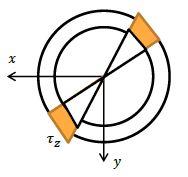
\includegraphics[width=0.55\linewidth]{figures/screenshot001}
	 	\label{fig:screenshot001}
	 \end{figure}
	 L'accoppiamento vite-dado prevederà anche l'utilizzo di rosette. 
	 
	 Quelle classiche aiutano a redistribuire la pressione: siccome la rigidezza di contatto è proporzionale alla superficie di contatto tra le piastre e tra testa-piastra, allora ingrandire la superficie di contatto  sulla piastra attraverso la rosetta permette di accrescere le prestazione della giunzione. 
	 
	 In alcuni casi la rosetta è elastica, utile ad avere una spinta sul dado e diminuire le probabilità di auto svitamento. 
	 
	 Un altro sistema anti-svitamento può essere il controdado: la pressione che si instaura tra i filetti quando si va ad includere il secondo dado, permette di avere una configurazione più salda. \newline 
	 
	 Il classico bullone è un sistema che viene montato  senza interferenza né contatto con le piastre: il foro realizzato sulle piastre è di dimensioni maggiori rispetto alla  dimensione massima d'ingombro con la vite, questo perché nelle condizioni ideali la vite deve lavorare esclusivamente a trazione. \newline 
	 
	 La classificazione delle vite segue uno standard costante  all'interno delle normative vigenti: questa viene infatti classificata con due numeri
	 \begin{enumerate}
	 	\item Il primo numero rappresenta la classe di resistenza a rottura. 
	 	\item Il secondo numero rappresenta il rapporto percentuale tra snervamento e rottura. 
	 \end{enumerate} 
	 Ad esempio per una vite classe 8.8, la resistenza a rottura è 
	 \[R_m = 8\times100 = \SI{800}{\mega\pascal}\]
	 Mentre il rapporto percentuale sarà pari all'80\% della rottura ovvero 
	 \[R_s = \SI{640}{\mega\pascal}\]
	Avere un secondo numero basso significa avere un'elevata riserva plastica ma una bassa resistenza elastica, al contrario si avrà una ridottissima riserva plastica e un elevatissima resistenza a snervamento.
	
	Sopra la classe 8.8 le viti sono alto-resistenziali: rottura e snervamento sono molto elevati. \newline 
	
	I dadi invece hanno una numerazione che tiene conto esclusivamente della classe di resistenza a rottura. 
	\newpage 	
	Le normative danno anche i valori di riferimento per i laminati che debbano essere collegati tramite giunzioni bullonate 
	\begin{figure}[H]
		\centering
		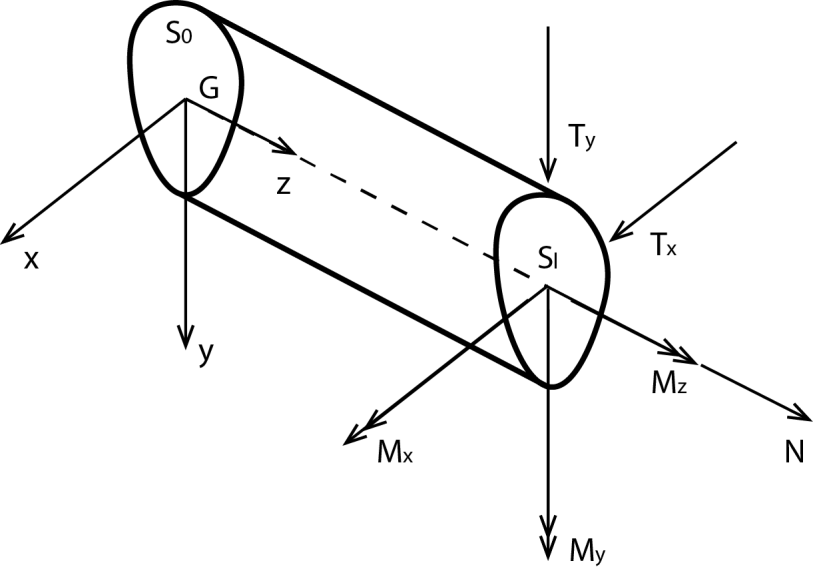
\includegraphics[width=0.8\linewidth]{figures/screenshot002}
		\caption{Resistenze minime da garantire}
		\label{fig:screenshot002}
	\end{figure}
	Se il materiale è meno resistente da quello indicato in normativa allora non può essere utilizzato. 
	
	$f_y$ è il limite di snervamento mentre $f_g$ è quello di rottura. 
	
	Ovviamente le tensioni ammissibili dei materiali non sono assolute e dipendono molto da come è stato realizzato l'oggetto base. 
	
	Se viene fornito in laminato, ha già subito delle lavorazioni che hanno fatto variare le dimensioni dei grani, avendo una struttura che da prestazioni  differenti rispetto al materiale bulk da fonderia. 
	
	Proprio per questo la normativa fornisce le caratteristiche in funzione dello spessore del materiale.  
\end{adjustwidth}
%\newpage
\subsection{Metodo delle tensioni ammissibili}
\begin{adjustwidth}{2in}{}	
	Per motivi di brevità non si affronterà la caratterizzazione del bullone in termini di rigidezza. 
	
	Per valutare il sistema di carichi transitanti sul giunto bullonato si dovrà valutare la rigidezza assiale del bullo alla quale si sommano le rigidezze delle piastre: per valutare  il sistema di rigidezze fornito dalla piastra si deve valutare la superficie di contatto effettivo tra le piastre magari considerando dei coni di influenza sulla piastra e considerando le rigidezze della piastra in parallelo a quelle della vite. \newline 
	
	Ciò che interessa in questa parte di corso è come si verificano i bulloni, come si scelgono secondo la classica UNI10011. \newline 
	
	Si fa il dimensionamento della giunzione esclusivamente a taglio, indipendentemente dai carichi transitanti sul bullone. \newline
	
	Questo è il caso in cui un giunto bullonato venga sollecitato nella direzione della piastra e vi sia uno scorrimento delle piastre  tale da portare a contatto dei semicilindri di ciascun foro. 
	 \begin{figure}[H]
	 	\centering
	 	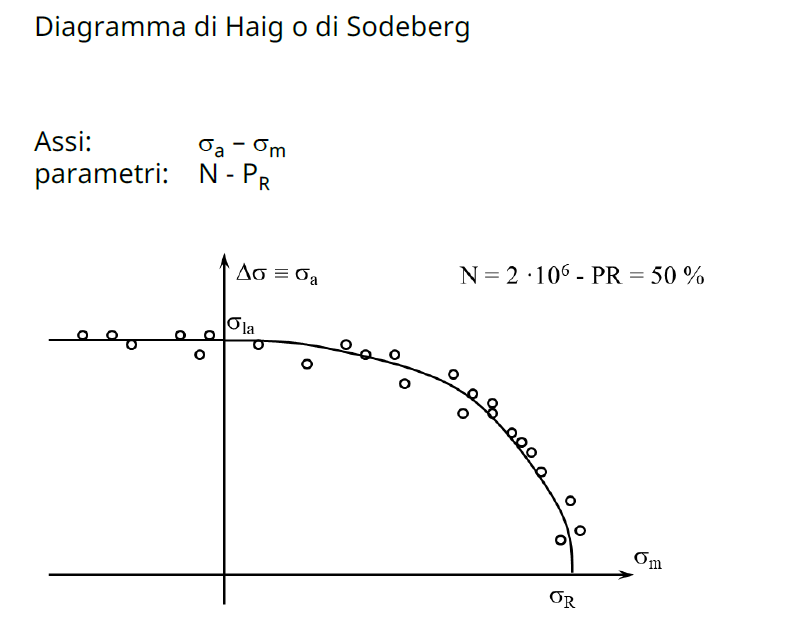
\includegraphics[width=0.7\linewidth]{figures/screenshot003}
	 	\label{fig:screenshot003}
	 \end{figure}
	 Questa è una tipologia di fenomeno che accade per bulloni non montati con precarico, ovvero bulloni che son ostati  serrati esclusivamente per portare a contatto le parti tra loro, senza realizzare una compressione preliminare delle piastre dettata da un serraggio del dado oltre la condizione di semplice contatto fra le parti. 
	 
	 Il precarico si applica soltanto alle viti alto-resistenziali. \newline 
	 
	 Questa verifica deterministica si applica perciò soltanto ai bulloni normali. 
	 
	 A seguito  di un carico in una direzione, le piastre collegate mediante il bullone risposeranno con una resistenza nella direzione opposta. \newline 
	 
	 Il comportamento della giunzione è ovviamente non lineare perché si  instaurano a seguito di questa applicazione del carico delle possibili non linearità dovute allo scorrimento delle parti in contatto. 
	 
	 La giunzione arriverà al collasso secondo 3 tipologie di danneggiamento.
	 \begin{figure}[H]
	 	\centering
	 	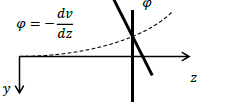
\includegraphics[width=0.7\linewidth]{figures/screenshot004}
	 	\label{fig:screenshot004}
	 \end{figure}
	 \begin{enumerate}
	 	\item Cedimento della vite a taglio;
	 	\item Rifollamento della piastra: le pressioni di contatto sulla piastra nel generano un cedimento locale;
	 	\item Cedimento della sezione resistente rimasta della piastra. 
	 \end{enumerate}
	 Nel parlare dell'approccio deterministico alla resistenza di un bullone si introducono una serie di ipotesi semplificative come 
	 \begin{enumerate}
	 	\item Comportamento perfettamente elastico di bulloni e lamiere. 
	 	\item Non c'è trasferimento di carico per attrito: il bullone è collegato senza applicare un'eccessiva pressione tra le parti. 
	 	\item Il gambo è sottoposto a sole azioni di taglio.
	 \end{enumerate}
	 Al fine di evitare la flessione secondario del giunto, è buona norma verificare che il carico sul bullone sia simmetrico lungo l'asse. 
	 \begin{figure}[H]
	 	\centering
	 	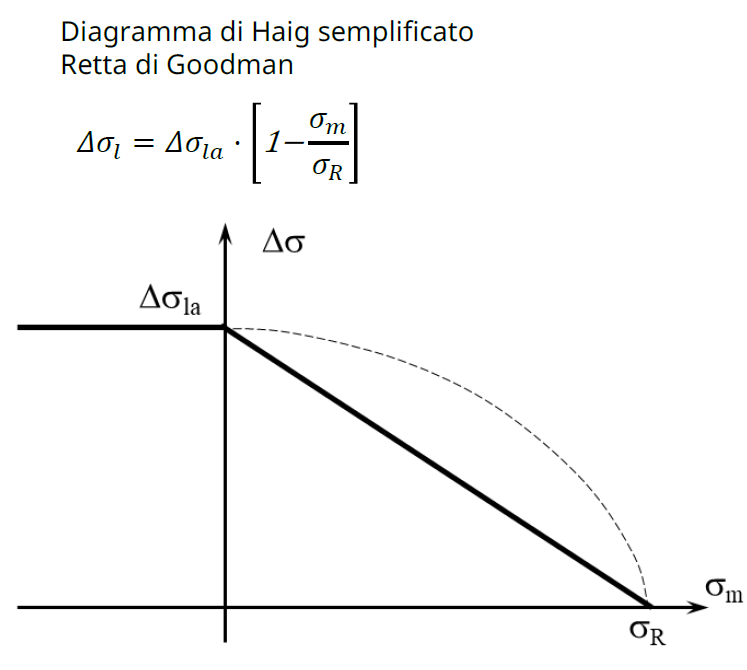
\includegraphics[width=0.5\linewidth]{figures/screenshot005}
	 	\caption{Buone pratiche di dimensionamento}
	 	\label{fig:screenshot005}
	 \end{figure}
\end{adjustwidth}
%\newpage
\subsubsection{Verifica a taglio}
\begin{adjustwidth}{2in}{}	 	 
	 Lavorando esclusivamente in ambito statico, si ipotizza che il carico della lamiera venga ripartito in modo uniforme su tutti i bulloni presenti nel giunto
	 \begin{figure}[H]
	 	\centering
	 	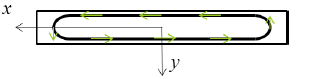
\includegraphics[width=0.7\linewidth]{figures/screenshot006}
	 	\caption{Giunto a 4 bulloni}
	 	\label{fig:screenshot006}
	 \end{figure}
	 Il carico $F$ è trasferito sui bulloni con una forza pari ad $F\over4$, mentre sulle altre lamiere viene ripartito in $F\over2$ e quindi in $F\over8$ sui fori corrispondenti. 
	 
	 La tensione di taglio sarà data, secondo normativa UNI, come il rapporto tra il carico transitante sul bullone ed il prodotto tra il numero di piani di taglio della piastra considerata e l'area resistente del bullone. 
	 \[\tau_b = \dfrac{R_b}{nA_{r,b}}\]
	 Quindi se si considera la piastra centrale si avranno due piani di carico, lavorando con la lamiera superiore si avrebbe un piano di carico.
	 
	 Il calcolo a resistenza della vite è identico se si usa la lamiera centrale o quelle superiori. 
	 
	 Ciò che è importante sottolineare è il denominatore. 	
\begin{figure}[H]
	\centering
	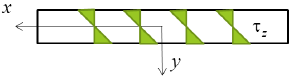
\includegraphics[width=0.7\linewidth]{figures/screenshot007}
	\label{fig:screenshot007}
\end{figure}
	L'area resistente del bullone, in condizioni statiche per materiale duttile, si trascura qualunque concentrazione di tensione, tuttavia si considera una differente area resistente in funzione di quale sia la sezione di  contatto tra la piastra la vite. 
	
	Se si sta valutando una piastra che tocca la vite nella parte non filettata, allora la sezione resistente sarà 
	\[\dfrac{\pi d^2}{4}\] 
	Se invece il bullone è tutto filettato, il contatto si avrà giocoforza sulla parte filettata e l'area resistente sarà pari a 
	\[\dfrac{\pi d_{res}^2}{4}\]
	In cui il diametro resistente, secondo normativa, è pari alla media tra il diametro di nocciolo ed il diametro medio della vite. 
	
	Questo fornisce un approccio equivalente per valutare il rapporto tra la riduzione di sezione ed il materiale resistente della vite.  
\end{adjustwidth}
\newpage
\subsubsection{Verifica delle piastre}
\begin{adjustwidth}{2in}{}	 		
	In realtà non si valuta esclusivamente la resistenza della vite per garantire la resistenza del giunto, infatti interessa il sistema nella sua interezza, il giunto compreso delle flange e dei bulloni, si dovrà verificare anche  la resistenza dell'oggetto collegato mediante bullone, il quale risulterà indebolito dalla presenza del foro.  
	\begin{figure}[H]
		\centering
		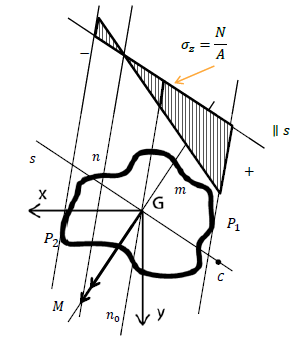
\includegraphics[width=0.7\linewidth]{figures/screenshot008}
		\label{fig:screenshot008}
	\end{figure}	
	Nell'approccio deterministico per materiale duttile e sollecitazione statica prevede sostanzialmente si utilizzare la tensione nominale. \newline 
	
	Quindi considerando il rapporto tra carico transitante sulla PIASTRA e la minima sezione resistente. 
	\[\sigma = \dfrac{F_v}{A_{nom}}\]
	Dove l'area nominale è data da 
	\[A_{nom} = (L-n\Phi)\cdot\text{sp}\]
	Il diametro del foro è sempre maggiore del diametro della vite: si deve permettere il passaggio senza danneggiare la filettatura. 
	
	Per piccoli diametri della vite il foro è semplicemente è pari ad \SI{1}{\milli\meter} in più rispetto al diametro della vite. 
	
	Per diametri superiori ai \SI{20}{\milli\meter} il diametro del foro è pari al diametro della vite più \SI{1.5}{\milli\meter}. \newline 
	
	Manca ogni riferimento alle concentrazioni di tensioni locali, il calcolo viene fatto solamente per via nominale eventuali plasticizzazioni locali di un materiale duttile non danno troppi  problemi di resistenza. 
\end{adjustwidth}
\newpage
\subsubsection{Verifica a rifollamento}
\begin{adjustwidth}{2in}{}	
	Il rifollamento è quel fenomeno - che interessa le piastre - generato dalle pressioni di contatto  tra in gambo della vite ed il foro della piastra: è necessario verificare che la piastra non si deformi localmente in maniera eccessiva. 
	\begin{figure}[H]
		\centering
		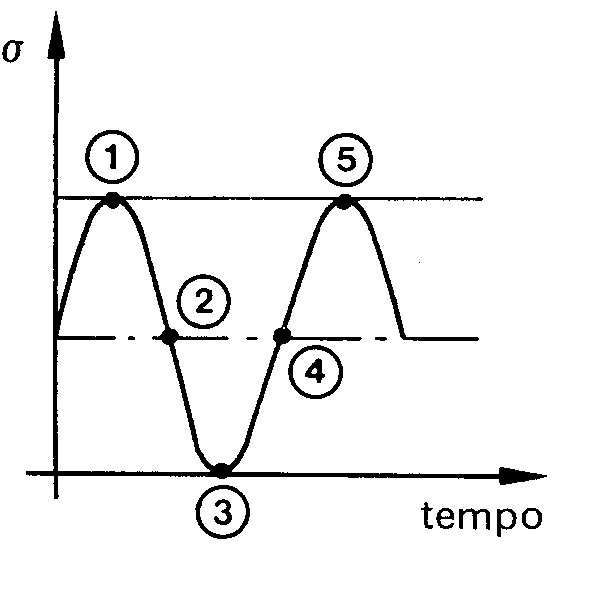
\includegraphics[width=0.7\linewidth]{figures/screenshot009}
		\label{fig:screenshot009}
	\end{figure}	
	La pressione che si instaura è una pressione hertziana la cui distribuzione è parabolica  dove il valore di massimo dipende dalle curvature dei materiali. \newline 
	
	Sempre in modo conservativo la normativa proporne un calcolo semplificato 
	\[\sigma_{rif} = \dfrac{R_b}{td}\]
	Ovvero il rapporto tra il carico transitante sulla piastra e la sezione normale alla piastra: prodotto tra diametro e spessore. 
	
	Questa pressione  così determinata dev'essere inferiore ad una tensione di riferimento, questa  dipendente dalle dimensioni della piastra, dal diametro del foro e dalla distanza del foro dal bordo della piastra nella direzione del carico, dipende ovvero dal rapporto 
	\[\alpha = \dfrac{a}{d}\approx 2\]
	Dove $a$ è la distanza dal bordo della piastra al centro foro nella direzione di transito del carico e $d$ è in diametro del foro. 
	
	L'ammissibile del materiale diventa così il doppio di quella utilizzata per la verifica a trazione della piastra. 
\end{adjustwidth}
\newpage
\subsubsection{Disposizioni costruttive}
\begin{adjustwidth}{2in}{}
	I calcoli finora effettuati riguardano il singolo bullone. 
	
	È vero che vale la sovrapposizione degli effetti - campo elastico - per cui la resistenza di un bullone può influenzare la resistenza del bullone affianco oppure l'indebolimento della piastra a seguito di un foro possa influenzare anche la sezione del bullone successivo. 
	
	Le formule finora utilizzate sono ancora validi finché esista una giusta spaziatura tra i fori dei bulloni. 
	
	I caso di non rispetto di tali indicazioni, si dovranno prevedere dei calcoli di dettaglio attraverso simulazioni FEM.  
	\begin{figure}[H]
		\centering
		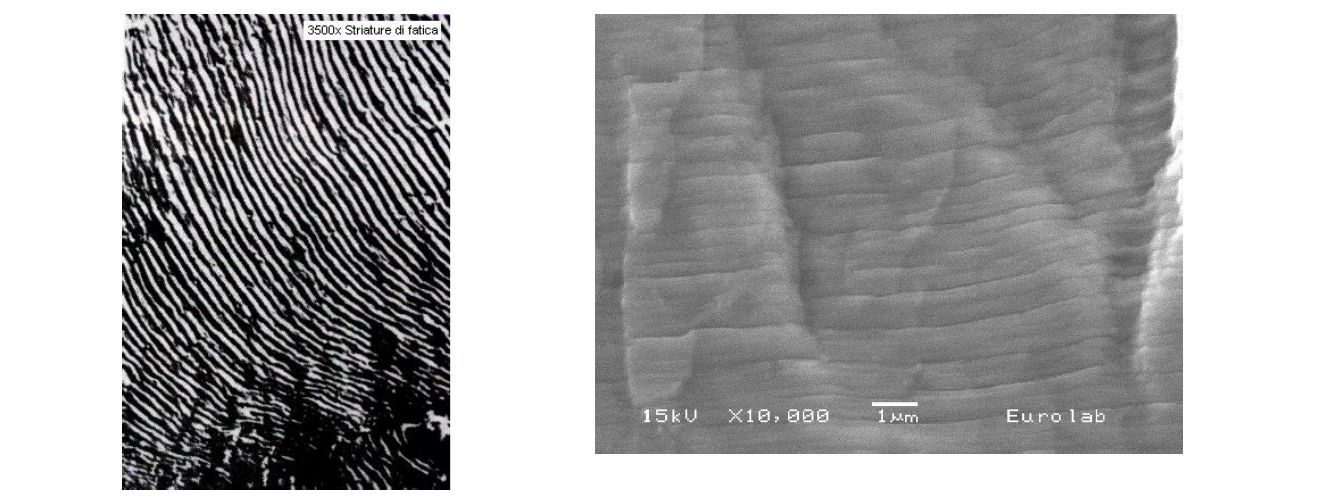
\includegraphics[width=0.7\linewidth]{figures/screenshot010}
		\label{fig:screenshot010}
	\end{figure}	
	La spaziatura è dettata sia da motivi di resistenza che funzionali al fine di garantire la presa con gli utensili. 
	
\end{adjustwidth}
\newpage
\subsection{Metodo degli stati limite}
\begin{adjustwidth}{2in}{}	
	Le recenti normative ricalcano sostanzialmente la normativa europea di riferimento UNIEN1993/EUROCODICE3. 
	
	Secondo queste normativi ci sono perciò due tipi di bullone, quelli che vanno precaricati e quelli che non vanno precaricati. \newline 
	
	I primi sono esclusivamente bulloni alto-resistenziali, mentre i secondi possono essere tutti, anche i suddetti. 
	
	Nel caso di bullone non precaricato l'azione di taglio sulle piastre è nulla:  in presenza di un carico nella direzione della piastra, queste scorrono liberamente fino a trovare l'ostruzione del gambo della vite dimensionando quest'ultima solamente a taglio. 
	
	Il precarico invece garantisce un comportamento completamente diverso del bullone: inserire un bullone significa avvitare intorno al suo asse un dado per farlo scorrere assialmente, se il bullone non è precaricato quest'azione porta al semplice contatto fra le parti, se invece si continua a serrare si va a creare una sorta di interferenza con la piastra andando a creare una forte compressione tra le parti. 
	 
	 Durante il montaggio il bullone è in contatto con le piastre soltanto mediante la testa de il dado e se il precarico è avvenuto correttamente, il bullone manterrà le posizione qualsiasi sia la forza applicata alla piastra, questo perché il carico generato dal precaricato ha sviluppato una forte forza normale tra le superfici di contatto con relativa azione di attrito, questa sarà la forza resistente che si oppone al carico della giunzione. \newline 
	 
	 In pratica sulla vite esiste esclusivamente un carico di trazione derivante dal serraggio del dado. \newline 
	 
	 Perché preferire un sistema precaricato ad uno non precaricato (entrambi opportunamente verificati)? 
	 
	 Una vite post sollecitazione a taglia una una forma irregolare, segno del fatto che il materiale ha scorso in una direzione. Se l'entità dello scorrimento è minore del gioco del foro, allora si riesce a smontare, altrimenti sarà complicato e difficile un suo possibile recupero, il vero sistema smontabile prevederà un precarico adeguato che mantenga in posizione le piastre senza che avvenga scorrimento. \newline 
	 
	 Quant'è il precarico adeguato? Il limite al precarico sarà quello sullo snervamento e sulla rottura del gambo della vite, la normativa corre  in soccorso dicendo che un precarico adeguato è tra il 70$\div$80\% dello snervamento. 
	 
	 Per quanto riguarda poi la manutenzione, questa sarà stagionale perché in dipendenza della temperatura: se il bullone avesse un $\alpha$ maggiore di quello delle piastre questo si allungherebbe e si perderebbe precarico; se invece il bullone avesse un $\alpha$ minore di quello delle piastre, durante la dilatazione termica aggiungerebbe precarico. 
\end{adjustwidth}
\newpage
\subsubsection{Disposizioni costruttive}
\begin{adjustwidth}{2in}{}	 
	L'eurocodice prende in considerazioni molti più aspetti delle uni già viste, come ad esempio per i bulloni disallineati. 
	\begin{figure}[H]
		\centering
		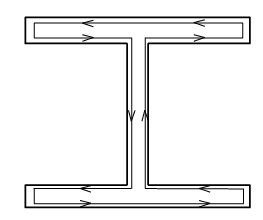
\includegraphics[width=0.7\linewidth]{figures/screenshot011}
		\label{fig:screenshot011}
	\end{figure}
\end{adjustwidth}
%\newpage
\subsubsection{Verifica a taglio}
\begin{adjustwidth}{2in}{}	
	Si inizia coi bulloni non precaricati, ossia solo quei bulloni che per garantire la resistenza della giunzione devono resistere a taglio. 	
	 \begin{figure}[H]
	 	\centering
	 	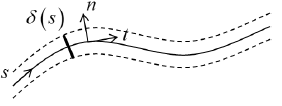
\includegraphics[width=0.7\linewidth]{figures/screenshot012}
	 	\label{fig:screenshot012}
	 \end{figure}
	 L'approccio semi-probabilistico ora impone una disuguaglianza tra carichi transitanti e non più tra tensioni locali. 
	 
	 A sinistra c'è la forza scambiata tra vite e singola piastra, mentre a destra vi sarà la resistenza a taglio della vite. 
	 
	 Tutti i fattori correttivi sono transitanti attraverso il solo termine a destra, è corretta coi fattori di sicurezza e quelli probabilistici. 
	 
	 Tant'è che si hanno tre possibilità di calcolo a seconda della classe del bullone. 
\end{adjustwidth}
\newpage
\subsubsection{Verifica a trazione degli elementi connessi}
\begin{adjustwidth}{2in}{}	 
	Il carico a trazione sull'elemento dev'essere inferiore al carico limite.
	
	Questo è preso come il minimo tra la resistenza plastica della sezione lorda (senza considerare la presenza dei fori) e la resistenza  a rottura della sezione nette, considerando una sezione ridotta dai fori. 
	\begin{figure}[H]
		\centering
		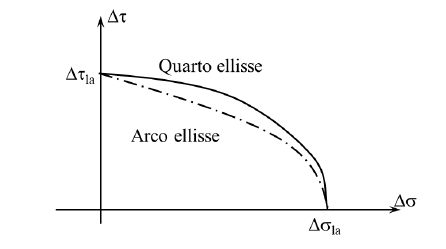
\includegraphics[width=0.7\linewidth]{figures/screenshot013}
		\label{fig:screenshot013}
	\end{figure}
\end{adjustwidth}
%\newpage
\subsubsection{Verifica a rifollamento}
\begin{adjustwidth}{2in}{}	
	Con la normativa precedente si era vista una sezione netta moltiplicata per un carico di rottura del materiale ed un fattore $\alpha$.Ora si aggiunge un fattore $k$ che tiene conto del bordo in direzione perpendicolare al carico, 	
	 \begin{figure}[H]
	 	\centering
	 	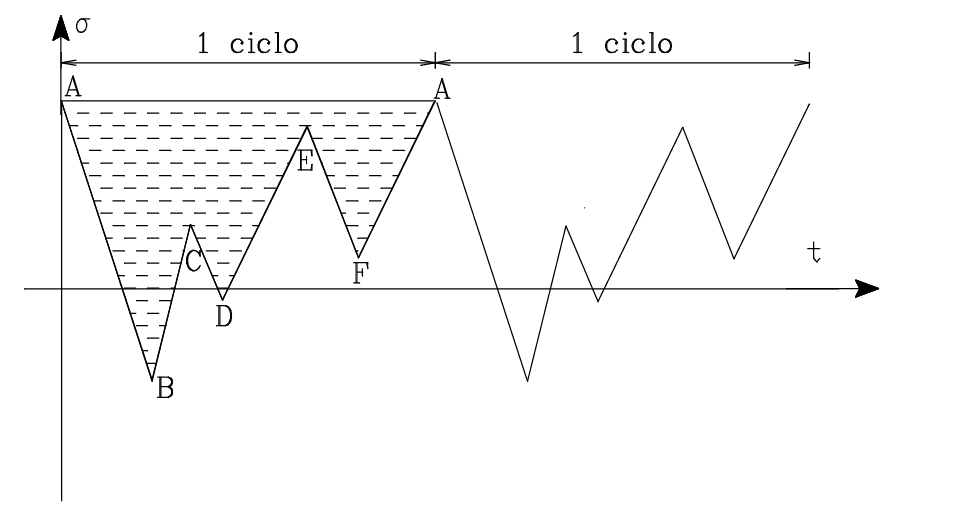
\includegraphics[width=0.7\linewidth]{figures/screenshot014}
	 	\label{fig:screenshot014}
	 \end{figure}
\end{adjustwidth}
\newpage
\subsubsection{Verifica a trazione dei bulloni}
\begin{adjustwidth}{2in}{}		 
	Questa normativa introduce infine un altro concetto. 
	\begin{figure}[H]
		\centering
		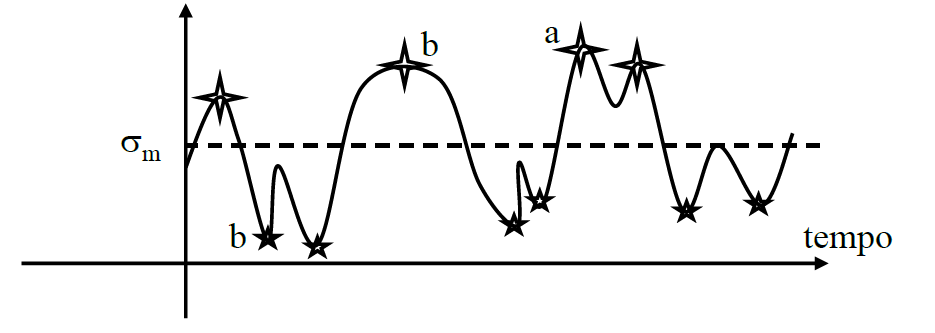
\includegraphics[width=0.7\linewidth]{figures/screenshot015}
		\label{fig:screenshot015}
	\end{figure}	
	Anche un bullone non precaricato potrebbe essere soggetto a trazione perché se il componente specifico viene trazionato, il carico si trasferisce anche sui bulloni. 
	
	Con questa verifica si deve garantire semplicemente di non arrivare alla rottura del materiale. 
\end{adjustwidth}
%\newpage
\subsubsection{Verifica a punzonamento degli elementi connessi}
\begin{adjustwidth}{2in}{}	
	C'è un'altra eventualità da valutare: se si ammette la trazione tra le viti, può accadere un altro fenomeno che accade. 
	\begin{figure}[H]
		\centering
		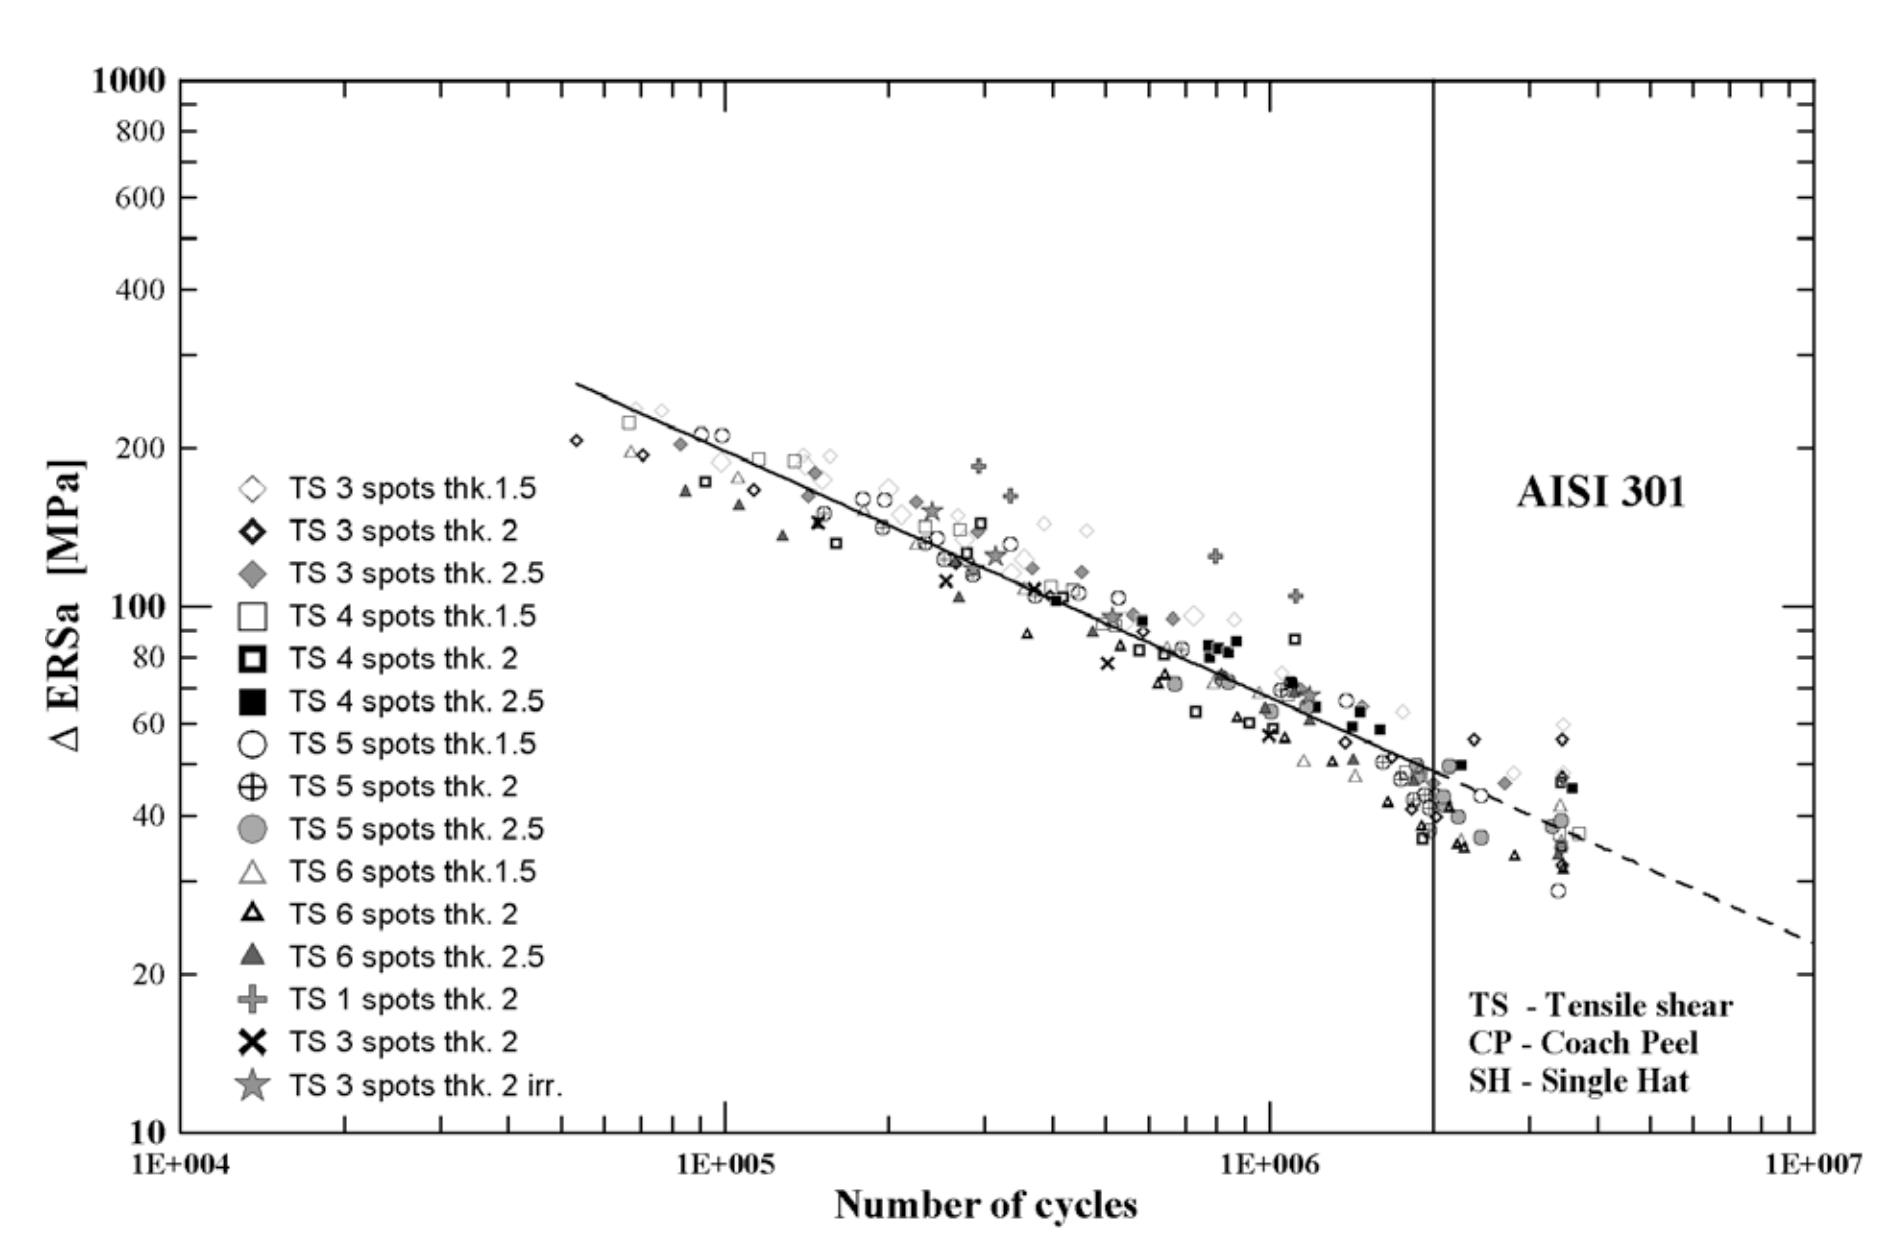
\includegraphics[width=0.7\linewidth]{figures/screenshot016}
		\label{fig:screenshot016}
	\end{figure}
	Se si mette in trazione il sistema, la superficie della piastra può subire una flessione importante. 
	
	Nelle superfici di contatto si creano delle forti concentrazioni di tensione che portano a deformare localmente la piastra, dato che la testa è molto più ampia rispetto al foro, questa lascia un'impronta sulla piastra che tende a danneggiarsi, provocando il punzonamento della piastra. 
	
	Nella relazione proposta a sinistra c'è il carico di trazione della vite mentre a destra c'è la resistenza a funzionamento del piatto 
\end{adjustwidth}
\newpage
\subsubsection{Verifica dei bulloni con stato di sollecitazione composto}
\begin{adjustwidth}{2in}{}	
	Con una situazione composta (come avviene nella quasi totalità dei bulloni) allora la verifica sarà "mischiata" applicando una combinazione lineare delle verifiche. 
		\begin{figure}[H]
			\centering
			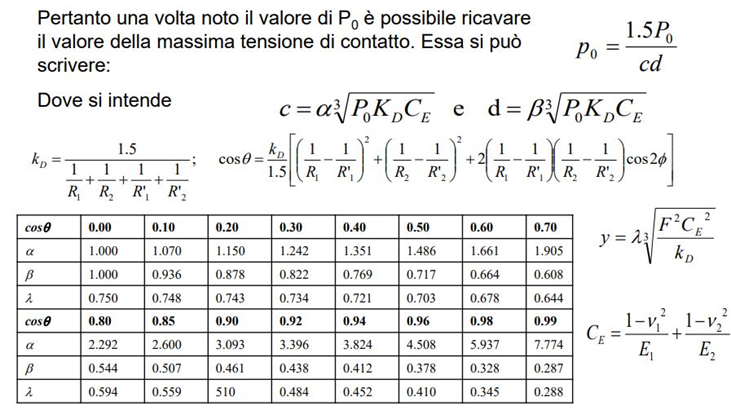
\includegraphics[width=0.7\linewidth]{figures/screenshot017}
			\label{fig:screenshot017}
		\end{figure}
		Naturalmente, la singola resistenza deve essere rispettata. 
\end{adjustwidth}
%\newpage
\subsubsection{Unioni a taglio con bulloni ad alta resistenza}
\begin{adjustwidth}{2in}{}	
	Il bullone precaricato, come già più volte detto, si distingue da quello normale per le condizioni di serraggio iniziale. 
	
	Esisterà per ciò una relazione che leghi la resistenza del giunto, con il carico transitante, ovvero una condizione di non-scorrimento del giunto precaricato. 
	
	Qualora questa condizione sia rispettata, non transita per il bullone altro carico se non il precarico. 
	
	Se invece avviene lo scorrimento o è stato scelto male il precarico oppure da quel momento in poi i calcoli dovranno essere effettuati esattamente come un bullone non precaricato. 
	\begin{figure}[H]
		\centering
		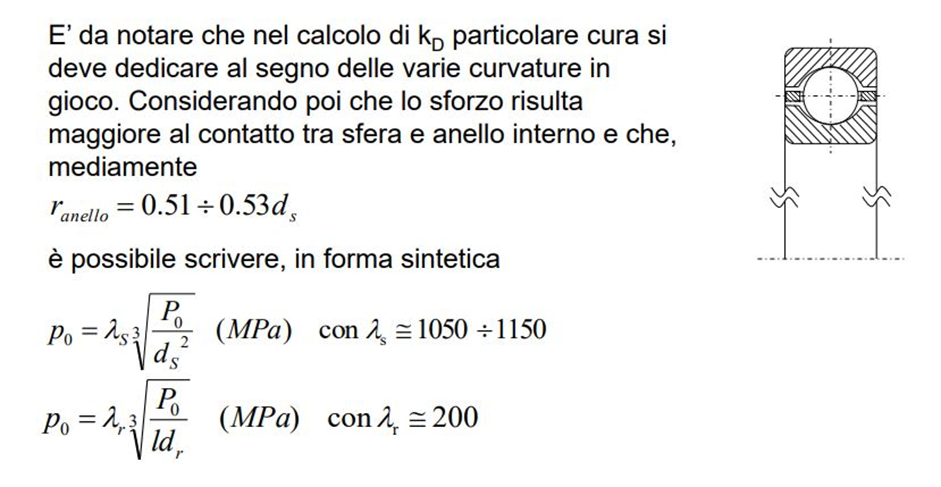
\includegraphics[width=0.7\linewidth]{figures/screenshot018}
		\label{fig:screenshot018}
	\end{figure}
	La verifica non è complessa, il carico  effettivamente transitante sul bullone deve essere inferiore a quello di resistenza, quest'ultima sarà data dal prodotto del numero di superfici di attrito per un coefficiente di attrito per il carico d'attrito (valore del precarico).
	
	Questo è il carico che genera sul gambo una trazione pari al 70\% dell'UTS.  \newline 
	
	Come si fa a sapere se è stato generato esattamente quel carico sul bullone? Si deve tradurre il carico in una coppia di serraggio, cioè un momento torcente ad applicare al dado che porti ad avere quel carico assiale: chiave dinamometrica. 
	
	Se invece il sistema non è controllato si dovrà applicare un fattore di sicurezza aggiuntivo. \newline 
	
	La normativa - che non è un manuale da officina - non fornisce la relazione tra precarico e coppia di serraggio: è un sistema complesso di molle in parallelo, gambo della vite, piastre serrate... All'avanzamento del dado resiste sia la compressione delle  piastre che la trazione del bullone, senza considerare le rigidezze ed i cedimenti locali dei punti di contatto testa-dado-piastre. \newline
	
	Tuttavia questa normativa non tiene in considerazione il sovraccarico di trazione: lo stato di trazione non rimane lo stesso ma si somma uno stato tensionale aggiuntivo, per cui se si era già sfruttato il 70\% della rottura, la tensione aggiuntiva (in elasticità lineare si può fare sovrapposizione degli effetti)  va sommato al 70\% per non raggiungere la rottura. 
\end{adjustwidth}
\newpage
\section{Saldature}
\begin{adjustwidth}{2in}{}
	Le tecniche di saldatura prevedono sempre una variazione locale delle caratteristiche meccaniche del materiale, questo perché viene portato a temperature prossime a quelle di fusione ed è costretto a solidificare in una posizione introducendo delle discontinuità di materiale, di caratteristiche meccaniche e delle concentrazioni di tensione, oltre alla presenza di intagli, porosità...
	
	In generale la saldatura è un punto di debolezza e di possibile cedimento. \newline 
	
	Un componente meccanico ha un buon design se è in grado di minimizzare le saldature presenti. \newline 
	
	Il processo di saldatura è tecnologicamente molto semplice, tuttavia l'esito della saldatura è legato all'esperienza dell'operatore e al livello tecnologico delle attrezzature. \newline 
	
	Il cordone di saldatura può essere composto di solo materiale d'apporto, di una legna tra materiale d'apporto e quello di base o di solo materiale di base e non è il solo ad avere caratteristiche meccaniche variabili, anche nella zona d'intorno, (ZTA) ci saranno tensioni residue indotte dal raffreddamento locale non controllato.
	
	Se poi il cordone viene lavorato alle macchine utensili per rientrare nelle tolleranze geometriche, ecco che si verranno  ad aggiungere tensioni residue dovute alle lavorazioni. \newline 
	
	la valutazione delle tensioni residue in un cordone di saldatura è un discorso complesso e sperimentale.\newline 
	
	Un progettista meccanico allora come si muove in questo senso? 
	
	Si utilizzano approcci semplificato che abbiano una buone dose di conservatività si valuteranno nominalmente le tensioni.\newline 
	
	La normativa di riferimento è la UNI10011 e valuta il cordone come una parte di struttura perfettamente continua con la lamiera  e priva di qualsivoglia concentrazioni di tensione e valuta esclusivamente le sollecitazioni statiche. \newline 
	
Le classi di saldatura  vengono valutate in funzione del tipo di controllo che viene fatto sulla saldatura (visivo - classe2, strumentato - classe1). \end{adjustwidth}
%\newpage
\subsection{Saldature a completa compenetrazione}
\begin{adjustwidth}{2in}{}
	Il materiale d'apporto  è inserito per tutta la profondità della lamiera, sia che la saldatura sia di testa che a T. 
	\begin{figure}[H]
		\parbox{0.45\textwidth}{\centering
		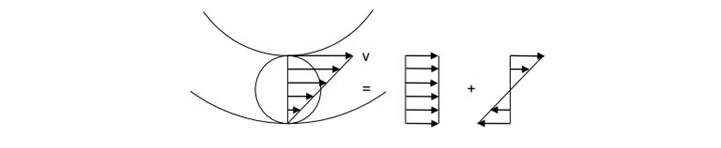
\includegraphics[width=0.5\linewidth]{figures/screenshot019}
		\label{fig:screenshot019}}
		\parbox{0.45\textwidth}{\centering
		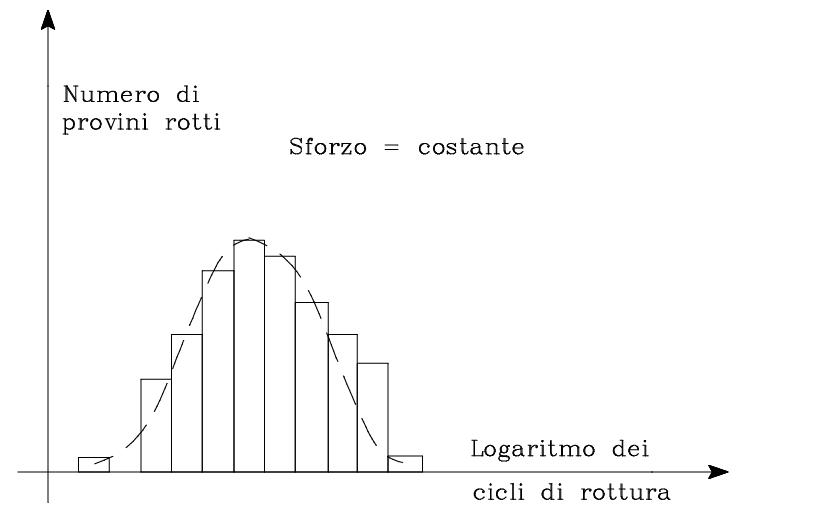
\includegraphics[width=0.5\linewidth]{figures/screenshot020}
		\label{fig:screenshot020}}
	\end{figure}
\begin{figure}[H]
	\centering
	\label{fig:screenshot021}
	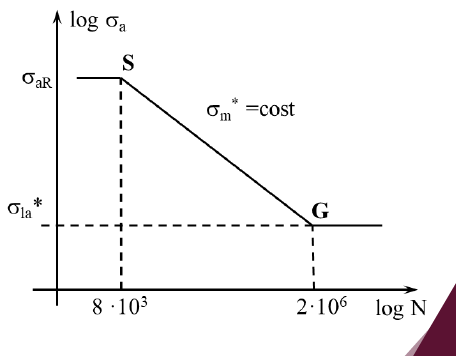
\includegraphics[width=0.2\linewidth]{figures/screenshot021}
\end{figure}
A seconda della classe di saldatura, l'ammissibile da utilizzare sarà tal quale (C1) o ridotto di un fattore 0.85 (C2). \newline 

La normativa prevede tre tipologie di tensioni transitanti sulla saldatura:, due tensioni nominali normali
\begin{itemize}
	\item $\sigma_{\perp}$ Tensione ortogonale al cordone di saldature
	\item $\sigma_{\parallel}$ Tensione parallela a cordone di saldatura
\end{itemize}
In più valuta delle $\tau_{\parallel}$ parallele al cordone di saldatura. 

Nel caso del cordone a T, la $\sigma_{\perp}$ è sempre perpendicolare al cordone ma in direzione della lamiera che viene completamente compenetrata dalla saldatura mentre le $\sigma_{\parallel}$ e $\tau_{\parallel}$ non variano. \newline 

Per valutare queste tensioni è necessario considerare una sezione resistente della lamiera, per cui per le $\tau_{\parallel}$ e le $\sigma_{\perp}$ la sezione resistente sarà pari a 
\[A_{res} = a\cdot L \]
Con $a$ minimo degli spessori delle due lamiere per saldature di testa, mentre per quelle a T è lo spessore della lamiera che è stata completamente compenetrata dalla saldatura.  \newline 

Per quanto riguarda la $\sigma_{\parallel}$, la sezione resistente sarà 
\[A_{res} = a\cdot h \]
Dove $h$ dev'essere di volta in volta valutata è la larghezza data dalla somma di quella del materiale di base e quello d'apporto. \newline 

Una volta ricavate queste tensioni, la tensione equivalente si comporrà esattamente con Von Mises
\[\sigma_{id} = \sqrt{\sigma_{\perp}^2 + \sigma_{\parallel}^2 - \sigma_{\perp}\sigma_{\parallel} + 3( \tau_{\perp} + \tau_{\parallel} )}\leq k_{1,2}\sigma_{amm}\]
\end{adjustwidth}
\newpage
\subsection{Saldature d'angolo}
\begin{adjustwidth}{2in}{}
	In un giunto a T con cordone d'angolo la saldatura è perfettamente esterna alle due lamiere.
   \begin{figure}[H]
   	\centering
   	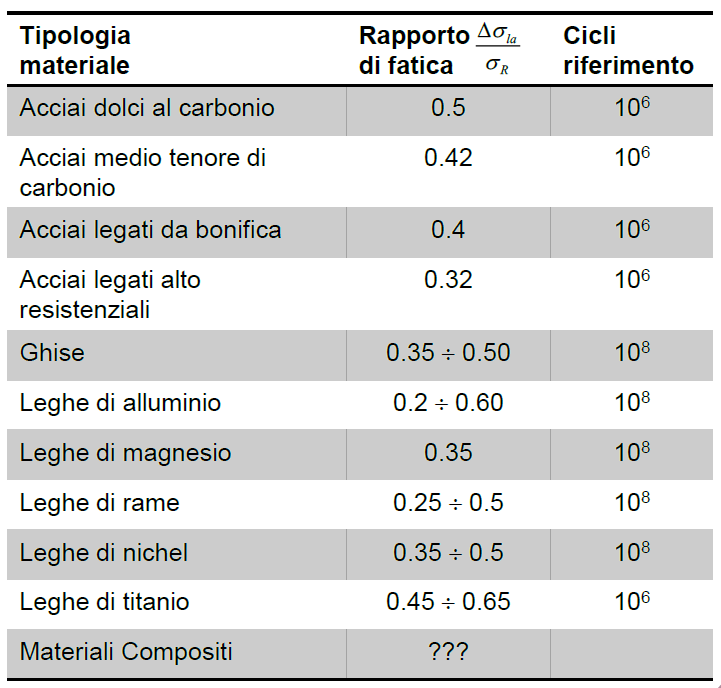
\includegraphics[width=0.2\linewidth]{figures/screenshot022}
   	\label{fig:screenshot022}
   \end{figure}
   Il coefficiente riduttivo $k_{1,2}$ della tensione ammissibile  dipende in questo caso esclusivamente dal materiale. \newline 
   
   Si possono avere vari tipi di cordoni d'angolo .
   \begin{figure}[H]
   	\centering
   	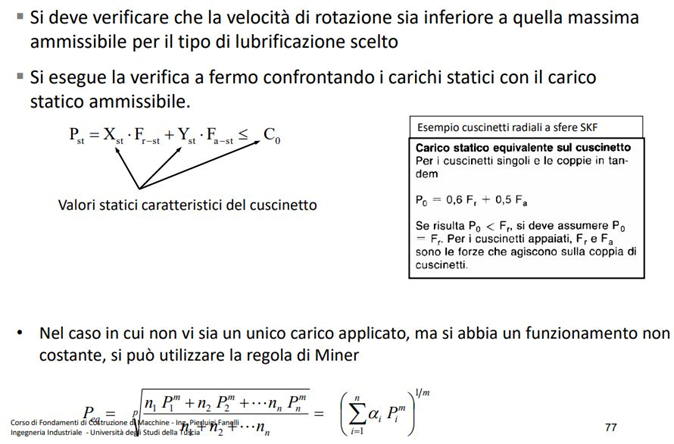
\includegraphics[width=0.2\linewidth]{figures/screenshot023}
   	\label{fig:screenshot023}
   \end{figure}
   La forma del cordone può dipendere sia dall'abilità dell'operatore, sia dalle caratteristiche del materiale d'apporto in base alla sua capillarità e alla sua aderenza. \newline 
   
   Si possono realizzare cordoni d'angolo per connettere lamiere parallele. 
   \begin{figure}[H]
   	\centering
   	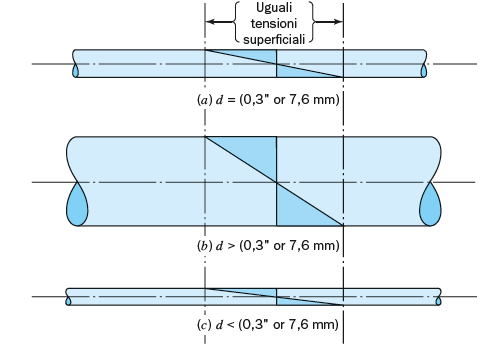
\includegraphics[width=0.2\linewidth]{figures/screenshot024}
   	\label{fig:screenshot024}
   \end{figure}
   Per garantire la resistenza, è buona norma realizzare il cordone non solo sopra come da immagine, ma anche sotto. \newline 
   
   Il cordone di saldatura può essere posto ortogonale o parallelo alla direzione del carico.\newline 
   
   La sezione resistente per questo tipo di saldature è pari a
   \[A_{res} = a\cdot L\]
   Con $L$ lunghezza del cordone ed $a$ minima sezione della gola: è l'altezza del triangolo inscrivibile nella sezione del cordone.\newline 
   
   La normativa dice che le tensioni da prendere in considerazione sono sempre 3, questa volta una normale e due tangenziali.  
   
   la $\sigma_{\parallel}$ nella direzione del cordone non è da prendere in considerazione perché in quella direzione  le forze sono scambiate soltanto per taglio, essendo il cordone sovrapposto alle lamiere, un carico sulla lamiera viene trasferito sull'altra attraverso l'azione di taglio del cordone, non attraverso la trazione/compressione del cordone. \newline 
   
   Si avranno perciò una $\sigma_{\perp}$ una $\tau_{\perp}$ ed una $\tau_{\parallel}$ tutte rispetto alla  sezione resistente ribaltata su una lamiera o sull'altra.
   \begin{figure}[H]
   	\centering
   	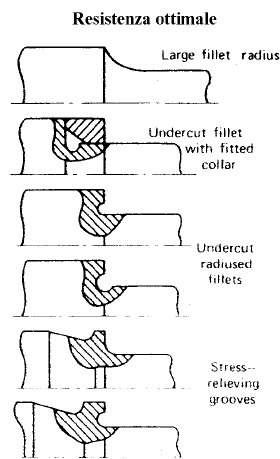
\includegraphics[width=0.5\linewidth]{figures/screenshot025}
   	\label{fig:screenshot025}
   \end{figure}
   \begin{figure}[H]
   	\centering
   	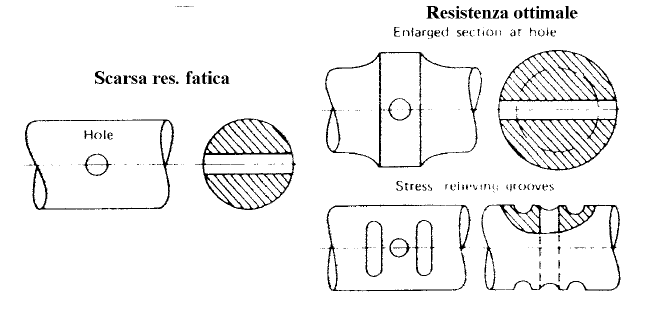
\includegraphics[width=0.5\linewidth]{figures/screenshot026}
   	\label{fig:screenshot026}
   \end{figure}
   Qualora il cordone non abbia una buona finitura alle estremità del cordone, è buona norma ridurre la sezione resistente di una quantità $a$ all'inizio e alla fine del cordone. \newline 
   
   In funzione  del tipo di acciaio si avrà un fattore correttivo sull'ammissibile. 
   
   La tensione ideale viene trattata attraverso una formulazione simil-Von Mises, deve sempre essere confrontata con la tensione ammissibile opportunamente scalata. 
   \begin{figure}[H]
   	\parbox{0.45\textwidth}{\centering
   	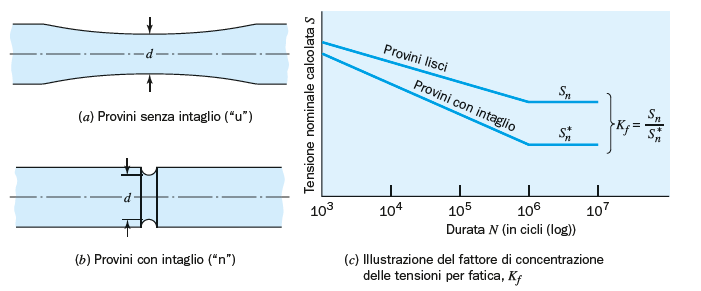
\includegraphics[width=1\linewidth]{figures/screenshot027}
   	\caption{Acciai basso-resistenziali}
   	\label{fig:screenshot027}}
   	\parbox{0.45\textwidth}{\centering
   	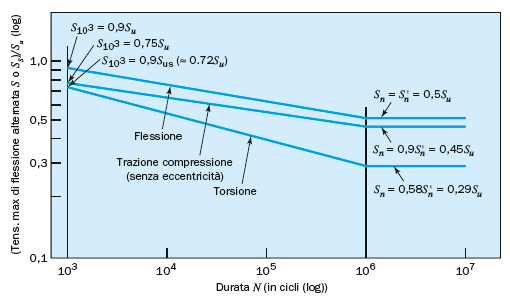
\includegraphics[width=1\linewidth]{figures/screenshot028}
   	\caption{Acciai alto-resistenziali}
   	\label{fig:screenshot028}}
   \end{figure}
   I minori coefficienti $k_i$ per acciai più resistenti sono dovuti al fatto che questi hanno maggiore sensibilità all'intaglio. 
   
 \newpage
 
 Nel caso in cui si avesse  almeno una delle tre tensioni nulle, il set di verifiche varia leggermente. 
 \begin{figure}[H]
 	\centering
 	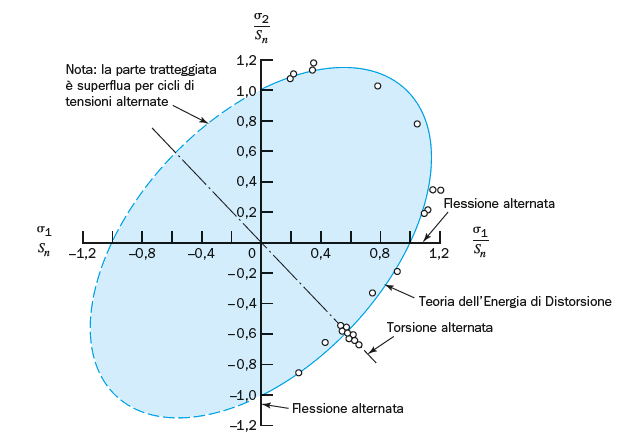
\includegraphics[width=0.7\linewidth]{figures/screenshot029}
 	\label{fig:screenshot029}
 \end{figure}
\end{adjustwidth}
\newpage
\subsection{Calcolo delle tensioni}
\begin{adjustwidth}{2in}{} 
	Quelle finora trattate sono tensioni nominali svolte attraverso un calcolo semplificato. \newline 
	
	Si valutano tutte le parti presenti come rigide: le lamiere non hanno deformabilità, la sezione resistente è elusivamente quella del cordone di saldatura. 
	
	Si valuta il baricentro del cordone di saldatura e si valutano i carichi equivalenti che agiscono sul baricentro del cordone: è un trasferimento di carico attraverso un modello a parametri concentrati. 
	
	Dopodiché si calcoleranno tutte quelle grandezze utili al calcolo con DSV sul cordone di saldatura: area resistente, inerzia rispetto all'asse baricentrico ortogonale, inerzia polare. 
	
	Si è in grado a questo punto di costruirsi le caratteristiche della sollecitazione sul cordone e passare alla valutazione delle tensioni
	\[\sigma_{traz} = \dfrac{P}{A} \qquad \tau_{taglio} = \dfrac{T}{A} \qquad \sigma_{fless~x,y} = \dfrac{M}{I_{x,y}}h_{\max~x,y} \qquad \tau_{tors} = \dfrac{M_{tors}}{J_p}h_{\max}\]
	Questi valori devono essere studiati lungo tutte le sezioni del cordone che si ritengono critiche.  
\end{adjustwidth}
%\newpage
\paragraph{Aggiunte dell'Eurocodice}
\begin{adjustwidth}{2in}{} 	
	L'eurocodice 3 si occupa del design delle strutture metalliche. 
	\begin{figure}[H]
		\centering
		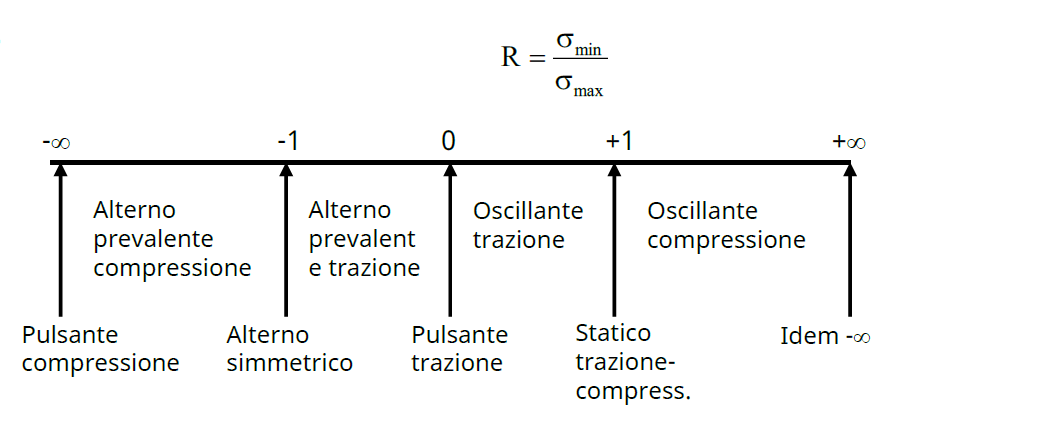
\includegraphics[width=0.7\linewidth]{figures/screenshot030}
		\label{fig:screenshot030}
	\end{figure}
	Per quanto riguarda le saldature a cordone d'angolo sussistono delle differenze rispetto alla normativa italiana. \newline 
	
	La verifica a resistenza si approccia in due modi diversi. 
	\begin{enumerate}
		\item \textbf{Metodo direzionale: approccio deterministico alle tensioni} \\
		Si considera come sezione resistente la minima sezione della gola, su cui agisce una terna di tensioni come in figura. \newline
		\begin{figure}[htp!]
			\centering
			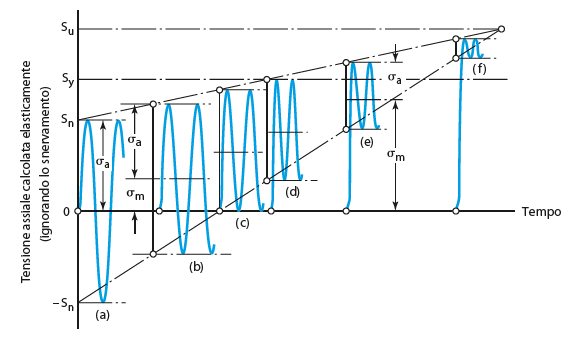
\includegraphics[width=0.5\linewidth]{figures/screenshot031}
			\label{fig:screenshot031}
		\end{figure}
		In questo caso la composizione delle tensioni prevede l'applicazione esatta di Von Mises
		\[\sqrt{\sigma_{\perp}^2 + 3(\tau_{\perp}^2 + \tau_{\parallel}^2)}\leq\dfrac{f_u}{\beta_W\gamma_{M2}}\]
		Con $\beta_W$ fattore  di correlazione tra materiale d'apporto e materiale di base. 
		\begin{figure}[H]
			\centering
			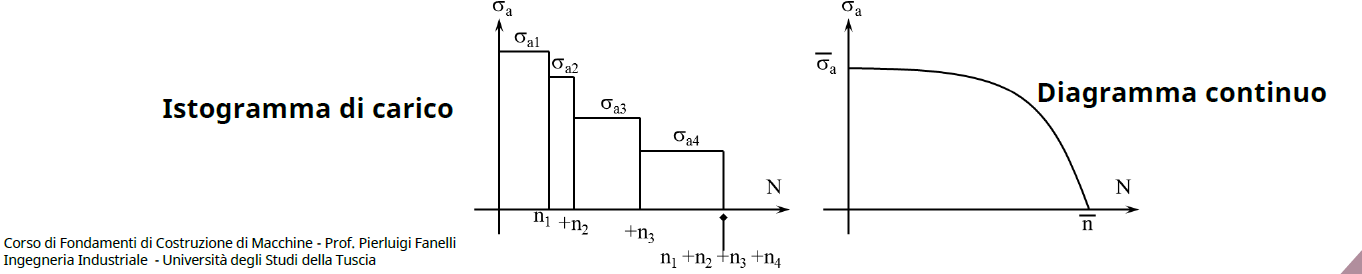
\includegraphics[width=0.5\linewidth]{figures/screenshot032}
			\label{fig:screenshot032}
		\end{figure}
		La più pericolosa delle tensioni, la $\sigma_{\perp}$ deve essere verificata singolarmente
		\[\sigma_{\perp} = 0.9\dfrac{f_u}{\gamma_{M2}}\] 
		
		\item \textbf{Approccio semi-probabilistico}\\
		Si valuta in questo vaso una forza risultante per unità di lunghezza sul cordone di saldatura, che debba essere confrontata con una forza resistente sempre per unità di lunghezza del cordone di saldatura. \newline 
		
		Questa forza resistente è data dalla resistenza a taglio della saldatura moltiplicata per una dimensione $a$, sezione minima della gola
		\[F_{W,Rd} = f_{vw,d}\cdot a = \dfrac{\dfrac{f_u}{\sqrt{3}}}{\beta_W\gamma_{M2}}\]			
		In 	questo modo però l'azione viene valutata come se fosse esclusivamente tagliante.
		\begin{figure}[H]
			\centering
			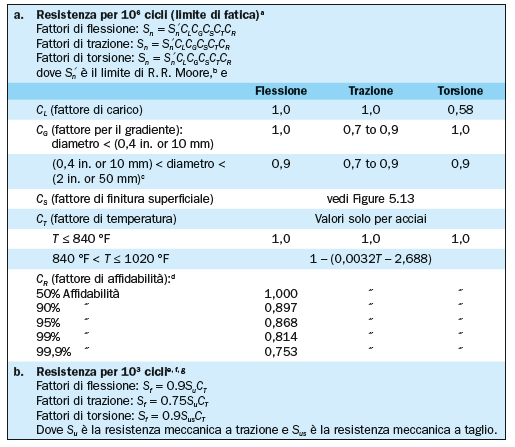
\includegraphics[width=0.7\linewidth]{figures/screenshot033}
			\label{fig:screenshot033}
		\end{figure}		 	
	\end{enumerate}
\end{adjustwidth}
\newpage
\subsection{Serie di esempi sulle slide: pp. 32-36}
\subsection{Fatica}
\begin{adjustwidth}{2in}{}	
	La fatica nell'eurocodice 3 vede un approccio notevolmente semplificato. 
	
	Si fa riferimento ad una variazione di tensione alternata intesa come $\Delta\sigma, \Delta\tau$ e anziché fare tutte quelle considerazioni sul ginocchio della curva, su cause, concause, parametri ed effetti della tensione media, si divide semplicemente i componenti meccanici per categorie.  	
	\begin{itemize}
		\item Giunti saldati di testa. 
		\item Giunti saldati per cordone d'angolo
		\item Giunti bullonati 
		\item Profilati scanalati
	\end{itemize} 
	A ciascun componente viene così assegnata una categoria di tensione $\Delta\Sigma_C$, cioè l'ammissibile - ad ampiezza costante - per un numero di cicli pari a \num{2d6}: fissa il ginocchio non più in funzione del materiale ma per quel determinato componente. \newline
	 
	Con la presenza di oscillazioni variabili si ammette l'utilizzo del metodo del serbatoio per valutare la tensione equivalente. \newline
	
	Il calcolo delle tensioni sulla la saldatura è analogo a quello delle sezioni statiche: si ribaltano le tensioni dov'è più comodo e si valutano le tensioni $\sigma, \tau$ parallele e perpendicolari. \newline 
	
	Queste tensioni dovranno essere confrontate con un diagramma di fatica simile.  
	\begin{figure}[H]
		\centering
		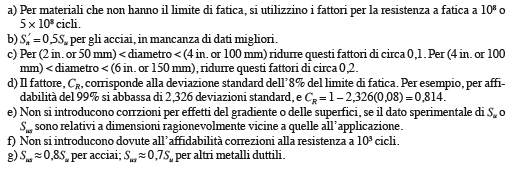
\includegraphics[width=0.7\linewidth]{figures/screenshot034}
		\label{fig:screenshot034}
	\end{figure}
	Le pendenze sono dettate da due coefficienti $m$ sempre uguali, dopo \num{10d8} cicli la vita a fatica è infinita. 
\newpage
La verifica si farà sempre con dei fattori di sicurezza attraverso gli approccio \textit{safe life} e \textit{damage tolerant}. 
\begin{figure}[H]
	\centering
	\includegraphics[width=0.7\linewidth]{figures/screenshot035}
	\label{fig:screenshot035}
\end{figure}
Spostando il ginocchio della curva di Wöhler per la determinata categoria. 
 \begin{figure}[H]
 	\centering
 	\includegraphics[width=0.7\linewidth]{figures/screenshot036}
 	\label{fig:screenshot036}
 \end{figure}
    
	
	
	   
	
	































\newpage
\textbf{{\LARGE NOTE}}
%	\vfill
%	\begin{tcolorbox}[height=4.5cm]
	%		This box has a height of 4.5cm.
	%	\end{tcolorbox}

%DA DECOMMENTARE PER AVERE LA VERSIONE STAMPABILE A DUE PAGINE 	
%	\newpage
%		\null
%		\vfill
%\begin{tcolorbox}[height=4.5cm]
%	This box has a height of 4.5cm.
%\end{tcolorbox}
%		
\end{adjustwidth}
\end{document}